\documentclass[10pt,aspectratio=169]{beamer}
\usetheme[progressbar=frametitle]{metropolis}
\usepackage{appendixnumberbeamer}

\usepackage{booktabs}

\usepackage{pgfplots}
% \usepgfplotslibrary{dateplot}

\usepackage{xspace}

% \newcommand{\themename}{\textbf{\textsc{metropolis}}\xspace}

\title{SLiM DIP: Indigo Snake Reintroduction}
% \date{\today}
\date{}
\author[shortname]{Matthew D. Buehler \inst{1} \and Noah Bevers \inst{2} \and Casey O'Neal \inst{2}}
\institute[shortinst]{\inst{1} Department of Biological Sciences \and \inst{2} Entomology Department}
% \titlegraphic{\hfill\includegraphics[height=1.5cm]{logo.pdf}}

\begin{document}

\maketitle

\begin{frame}{Table of Contents}
  \setbeamertemplate{section in toc}[sections numbered]
  \tableofcontents%[hideallsubsections]
\end{frame}


\section[Background]{Eastern Indigo Snake Background}
\begin{frame}{Eastern Indigo Snake Background}
\begin{columns}[c]
    \begin{column}[c]{5cm}
        \begin{itemize}
            \item Federally Threatened Species
            \item Extirpated in Alabama
            \item Ongoing re-introduction efforts
        \end{itemize}
    \end{column}
    \begin{column}[c]{10cm}
        \begin{figure}
            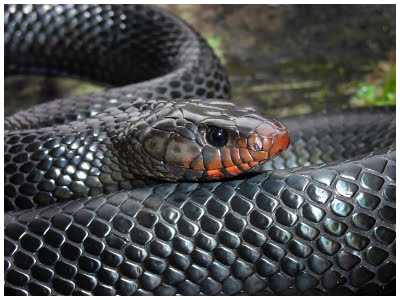
\includegraphics[height = 5cm]{media/indigo-snake-walton-outdoors.jpg}
        \end{figure}
    \end{column}
\end{columns}   
\end{frame}

\begin{frame}{Folt et al. (2019) - Extinction Models}
\begin{columns}
    \begin{column}[c]{5cm}
        \begin{itemize}
            \item Modeled the probabilty of extinctions for reintroduction efforts
            \item Found that 30 sub-adults over 10 years is the best case scenario
            \item Lacks any population genetics parameters
        \end{itemize}
    \end{column}

    \begin{column}[t]{8cm}
        \begin{figure}
            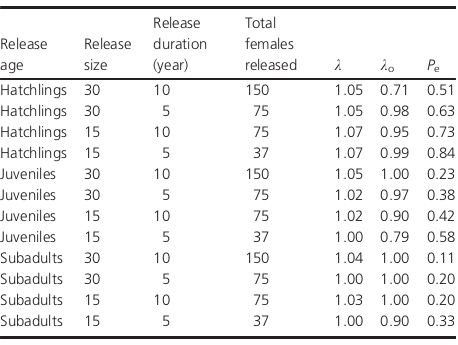
\includegraphics[height = 7cm]{media/folt-probabilities.png}
        \endP{figure}
    \end{column}
\end{columns}
\end{frame}



\end{document}
